
\documentclass[twoside,22pt]{Latex/Classes/thesisUMSNH}
%         PUEDEN INCLUIR EN ESTE ESPACIO LOS PAQUETES EXTRA, O BIEN, EN EL ARCHIVO "PhDthesisPSnPDF.cls" EN "./Latex/Classes/"
\usepackage{blindtext}                        % Para insertar texto dummy, de ejemplo, pues.
\usepackage{setspace}
\usepackage[round, sort, numbers]{natbib}  % Personalizar la bibliografía a gusto de cada quien
\usepackage{booktabs}
% Note:
% The \blindtext or \Blindtext commands throughout this template generate dummy text
% to fill the template out. These commands should all be removed when 
% writing thesis content.
% This file contains macros that can be called up from connected TeX files
% It helps to summarise repeated code, e.g. figure insertion (see below).

%%%%%%%%%%%%%%%%%%%%%%%%%%%%%%%%%%%%%%%%%%%%%%
%            Colores de la UNAM              %
%%%%%%%%%%%%%%%%%%%%%%%%%%%%%%%%%%%%%%%%%%%%%%
% Para UNAN: Azul Pantone 541  -->(0,63,119) RGB
% Para UMSNH: PANTONE Blue 072 C
\definecolor{Azul}{RGB}{51,51,153}

% Para UNAM: Oro Pantone 460  -->(234,221,150) RGB
% Para UMNSH: PANTONE 110 C
\definecolor{Oro}{RGB}{204,153,51}


%%%%%%%%%%%%%%%%%%%%%%%%%%%%%%%%%%%%%%%%%%%%%%
%            Comandos para líneas            %
%%%%%%%%%%%%%%%%%%%%%%%%%%%%%%%%%%%%%%%%%%%%%%
%Se define un comando \colorvrule para hacer líneas verticales de color con 3 argumentos: color, ancho, alto
\newcommand{\colorvrule}[3]{
\begingroup\color{#1}\vrule width#2 height#3
\endgroup}

%Se define un comando \colorhrule para hacer líneas horizontales de color con 2 argumentos: color, ancho
\newcommand{\colorhrule}[2]{
\begingroup\color{#1}\hrule height#2
\endgroup}

%%%%%%%%%%%%%%%%%%%%%%%%%%%%%%%%%%%%%%%%%%%%%%
%          Comando para derivadas            %
%%%%%%%%%%%%%%%%%%%%%%%%%%%%%%%%%%%%%%%%%%%%%%
\newcommand{\derivada}[3][]{\ensuremath{\dfrac{\mbox{d}^{#1}#2}{\mbox{d}#3^{#1}}}} 
%primer argumento(opcional): orden de la derivada
%segundo argumento: función a derivar
%tercer argumento: variable respecto a la que se deriva


%%%%%%%%%%%%%%%%%%%%%%%%%%%%%%%%%%%%%%%%%%%%%%
%       Comando para la exponencial          %
%%%%%%%%%%%%%%%%%%%%%%%%%%%%%%%%%%%%%%%%%%%%%%
\newcommand{\e}[1][]{\ensuremath{\mbox{e}^{#1}}}
%primer argumento(opcional): exponente de la exponencial




% insert a centered figure with caption and description
% parameters 1:filename, 2:title, 3:description and label
\newcommand{\figuremacro}[3]{
	\begin{figure}[htbp]
		\centering
		%% \includegraphics[width=3\textwidth]{#1}
		\caption[#2]{\textbf{#2} - #3}
		\label{condicion}
	\end{figure}
}

% insert a centered figure with caption and description AND WIDTH
% parameters 1:filename, 2:title, 3:description and label, 4: textwidth
% textwidth 1 means as text, 0.5 means half the width of the text
\newcommand{\figuremacroW}[4]{
	\begin{figure}[htbp]
		\centering
		%\includegraphics[width=#4\textwidth]{#1}
		\caption[#2]{\textbf{#2} - #3}
		\label{#1}
	\end{figure}
}

% inserts a figure with wrapped around text; only suitable for NARROW figs
% o is for outside on a double paged document; others: l, r, i(inside)
% text and figure will each be half of the document width
% note: long captions often crash with adjacent content; take care
% in general: above 2 macro produce more reliable layout
\newcommand{\figuremacroN}[3]{
	\begin{wrapfigure}{o}{0.5\textwidth}
		\centering
		\includegraphics[width=0.48\textwidth]{#1}
		\caption[#2]{{\small\textbf{#2} - #3}}
		\label{#1}
	\end{wrapfigure}
}

% predefined commands by Harish
\newcommand{\PdfPsText}[2]{
  \ifpdf
     #1
  \else
     #2
  \fi
}

\newcommand{\IncludeGraphicsH}[3]{
 \PdfPsText{\includegraphics[height=#2]{#1}}{\includegraphics[bb = #3, height=#2]{#1}}
}

\newcommand{\IncludeGraphicsW}[3]{
  \PdfPsText{\includegraphics[width=#2]{#1}}{\includegraphics[bb = #3, width=#2]{#1}}
}

\newcommand{\InsertFig}[3]{
  \begin{figure}[!htbp]
    \begin{center}
      \leavevmode
      #1
      \caption{#2}
      \label{#3}
    \end{center}
  \end{figure}
}







%%% Local Variables:
%%% mode: latex
%%% TeX-master: "~/Documents/LaTeX/CUEDThesisPSnPDF/thesis"
%%% End:
           % Archivo con funciones útiles

\usepackage[T1]{fontenc}
\usepackage[scaled]{uarial}
\renewcommand*\familydefault{\sfdefault} %% Only if the base font of the document	

\setlength{\parindent}{0cm}

%%%%%%%%%%%%%%%%%%%%%%%%%%%%%%%%%%%%%%%%%%%%%%%%%%%%%%%%%%%%%%%%%%%%%%%%%%%%%%%%
%                                   DATOS                                      %
%%%%%%%%%%%%%%%%%%%%%%%%%%%%%%%%%%%%%%%%%%%%%%%%%%%%%%%%%%%%%%%%%%%%%%%%%%%%%%%%
\title{ \textsc{DESARROLLO DE UN SISTEMA DE ALTO VOLTAJE PARA ACELERADORES DE PARTICULAS}}
\author{Juan Francisco Verdugo Arredondo} 
\facultad{Facultad de Ciencias Físico Matemáticas}   
\escudofacultad{Latex/Classes/Escudos/fmed_grande} % Aquí ponen la ruta y nombre del escudo de su facultad, actualmente, la carpeta Latex/Classes/Escudos cuenta con los siguientes escudos:
% "fi_azul" Facultad de ingenieria en color azul
% "fi_negro" Facultad de ingenieria en color negro
% "fc_azul" Facultad de ciencias en color azul
% "fc_negro" Facultad de ciencias en color negro

\degree{Licenciado en Electrónica}       % Carrera
\director{Carlos Duarte Galván \\ Christian Valerio Lizárraga}                  % Director de tesis
%\tutor{Nombre  Tutor }                    % Tutor de tesis, si aplica
\degreedate{2019}                                     % Año de la fecha del examen
\lugar{Culiacán, Sinaloa}                        % Lugar

%\portadafalse                              % Portada en NEGRO, descomentar y comentar la línea siguiente si se quiere utilizar
\portadatrue                                % Portada en COLOR



%% Opciones del posgrado (descomentar si las necesitan)
	%\posgradotrue                                                    
	%\programa{programa de maestría y doctorado en ingeniería}
	%\campo{Ingeniería Eléctrica - Control}
	%% En caso de que haya comité tutor
	%\comitetrue
	%\ctutoruno{Dr. Emmet L. Brown}
	%\ctutordos{Dr. El Doctor}
%% Datos del jurado                             
	%\presidente{Dr. 1}
	%\secretario{Dr. 2}
	%\vocal{Dr. 3}
	%\supuno{Dr. 4}
	%\supdos{Dr. 5}
	%\institucion{el Instituto de Ingeniería, UNAM}

\keywords{tesis,Juan Francisco Verdugo Arredondo,Carlos Duarte Galvan,acelerador de partículas}            % Palablas clave para los metadatos del PDF
\subject{acelerador de partículas,Física de altas energías}                     % Tema para metadatos del PDF  

%%%%%%%%%%%%%%%%%%%%%%%%%%%%%%%%%%%%%%%%%%%%%%%%%%%%%
%                   PORTADA                         %
%%%%%%%%%%%%%%%%%%%%%%%%%%%%%%%%%%%%%%%%%%%%%%%%%%%%%
\begin{document}
\begin{center}
{\Large \textsc{UNIVERSIDAD AUTÓNOMA DE SINALOA}}

\begin{Large}
\setlength{\parskip}{20pt}
FACULTAD DE CIENCIAS FÍSICO MATEMÁTICAS
\end{Large}


\setlength{\parskip}{60pt}

\begin{figure}[H]
\centering

\includegraphics[width=4cm]{logo.png}
\end{figure}
\setlength{\parskip}{20pt}

\begin{Large}
DESARROLLO DE UN SISTEMA DE ALTO VOLTAJE PARA ACELERADORES DE PARTÍCULAS 
\end{Large}

\setlength{\parskip}{40pt}
\begin{Huge}
T\hspace{1cm}E\hspace{1cm}S\hspace{1cm}I\hspace{1cm}S
\end{Huge}

\setlength{\parskip}{5pt}
\begin{normalsize}
QUE PARA OPTAR POR EL GRADO DE:
\end{normalsize}

\setlength{\parskip}{5pt}
\textbf{\begin{large}
Licenciado en electrónica
\end{large}}

\setlength{\parskip}{30pt}

\begin{large}
PRESENTA:
\end{large}

\setlength{\parskip}{5pt}
\textbf{\begin{large}
Juan Francisco Verdugo Arredondo
\end{large}}


\setlength{\parskip}{30pt}


\begin{normalsize}
DIRECTOR:\\
Dr. Carlos Duarte Galván\\
Dr. Cristhian Alfonso Valerio Lizarraga\\
\end{normalsize}


\setlength{\parskip}{60pt}
Culiacán, Sinaloa, 2019
\end{center}

\thispagestyle{empty}
\newpage
%\maketitle									% Se redefinió este comando en el archivo de la clase para generar automáticamente la portada a partir de los datos

%%%%%%%%%%%%%%%%%%%%%%%%%%%%%%%%%%%%%%%%%%%%%%%%%%%%%
%                  PRÓLOGO                          %
%%%%%%%%%%%%%%%%%%%%%%%%%%%%%%%%%%%%%%%%%%%%%%%%%%%%%




\begin{large}

\begin{dedication}
A mis padres, Martha Aidé Arredondo Solís y Francisco Verdugo Fierro.
A mis hermanos Dulce Esmeralda Verdugo Arredondo y Néstor Javier Espino Arredondo.
Por ayudarme a crecer en cada aspecto de mi vida.\\
Yo.
\end{dedication}
       % Comentar línea si no se usa
%\chapter*{}
%\pagenumbering{Roman}

\begin{acknowledgements}

También quiero agradecer a mis grandes maestros que me enseñaron que la sabiduría se encuentra en la motivación y el trabajo duro, Dr. Carlos Duarte Galvan, Dr. Cristian Alfonso Valerío Lizárraga, Dr. Jesús Roberto Millán Almaraz, etc..\\
A mi Universidad, sus instituciones y al personal administrativo, por abrirme las puertas a esta gran casa de estudio, al parque de innovación tecnológico, por haberme formado de la mejor manera posible y por la infinidad de oportunidades que se abren tras el conocimiento que se me ha otorgado. Sin mas ¡GRACIAS!
\end{acknowledgements}




   % Comentar línea si no se usa 
% ******************************* Thesis Declaration ********************************

\begin{declaration}

Por la presente declaro que, salvo cuando se haga referencia específica al trabajo de otras personas, el contenido de esta tesis es original y no se ha presentado total o parcialmente para su consideración para cualquier otro título o grado en esta o cualquier otra Universidad. Esta tesis es resultado de mi propio trabajo y no incluye nada que sea el resultado de algún trabajo realizado en colaboración, salvo que se indique específicamente en el texto. 
% Author and date will be inserted automatically from thesis.tex


\end{declaration}
           % Comentar línea si no se usa
%0
% Thesis Abstract -----------------------------------------------------


%\begin{abstractslong}    %uncommenting this line, gives a different abstract heading
\begin{abstracts}        %this creates the heading for the abstract page
El trabajo de esta tesis consiste en el desarrollo de la etapa de potencia de un acelerador de partículas lineal, el cual se centra en el diseño y construcción de una fuente de alto voltaje (HPS) basado en el sistema Cockcroft Walton  y un transformador de ignición capaz de suministrar 20 KV a 180 W, controlando el sistema digitalmente mediante un micro-controlador y comunicación Serial PC-HPS.\\☺

Durante el desarrollo de potencia se hizo el diseño, la simulación, la fabricación y la calibración de la electrónica y mecánica necesaria, optimizando así la precisión y costes del proyecto.\\*

Obteniendo como resultado un sistema de bajo coste, con el cual, mediante un computador se tiene la posibilidad de un control automatizado y  del sistema en general. 


\end{abstracts}
%\end{abstractlongs}


% ----------------------------------------------------------------------                   % Comentar línea si no se usa

\end{large}
%%%%%%%%%%%%%%%%%%%%%%%%%%%%%%%%%%%%%%%%%%%%%%%%%%%%%
%                   ÍNDICES                         %
%%%%%%%%%%%%%%%%%%%%%%%%%%%%%%%%%%%%%%%%%%%%%%%%%%%%%
%Esta sección genera el índice
\setcounter{secnumdepth}{3} % organisational level that receives a numbers
\setcounter{tocdepth}{3}    % print table of contents for level 3
\tableofcontents            % Genera el índice 
%: ----------------------- list of figures/tables ------------------------
\listoffigures              % Genera el ínidce de figuras, comentar línea si no se usa
%\listoftables               % Genera índice de tablas, comentar línea si no se usa


%%%%%%%%%%%%%%%%%%%%%%%%%%%%%%%%%%%%%%%%%%%%%%%%%%%%%
%                   CONTENIDO                       %
%%%%%%%%%%%%%%%%%%%%%%%%%%%%%%%%%%%%%%%%%%%%%%%%%%%%%
% the main text starts here with the introduction, 1st chapter,...
\mainmatter
\def\baselinestretch{1.5}                   % Interlineado de 1.5
%\doublespacings

\begin{large}


% this file is called up by thesis.tex
% content in this file will be fed into the main document
%----------------------- introduction file header -----------------------
%%%%%%%%%%%%%%%%%%%%%%%%%%%%%%%%%%%%%%%%%%%%%%%%%%%%%%%%%%%%%%%%%%%%%%%%%
%  Capítulo 1: Introducción- DEFINIR OBJETIVOS DE LA TESIS              %
%%%%%%%%%%%%%%%%%%%%%%%%%%%%%%%%%%%%%%%%%%%%%%%%%%%%%%%%%%%%%%%%%%%%%%%%%

%\chapter{Introducción}

%: ----------------------- HELP: latex document organisation
% the commands below help you to subdivide and organise your thesis
%    \chapter{}       = level 1, top level
%    \section{}       = level 2
%    \subsection{}    = level 3
%    \subsubsection{} = level 4
%%%%%%%%%%%%%%%%%%%%%%%%%%%%%%%%%%%%%%%%%%%%%%%%%%%%%%%%%%%%%%%%%%%%%%%%%
%                           Presentación                                %
%%%%%%%%%%%%%%%%%%%%%%%%%%%%%%%%%%%%%%%%%%%%%%%%%%%%%%%%%%%%%%%%%%%%%%%%%

\chapter{Resumen} % section headings are printed smaller than chapter names

El trabajo de esta tesis consiste en el desarrollo de una fuente de alto voltaje de bajo ruido para su uso en equipo científico de alta precisión, mediante la utilización  de un sistema de inversor de voltaje y un rectificador del tipo multiplicador, Cockcroft–Walton, así como también la introducción a un control del sistema con lazo cerrado e interfaces gráficas para el usuario.\\

Durante el desarrollo del sistema de alto voltaje se realizo el diseño, la simulación, la fabricación y la validación de los datos proporcionados por el sistema.\\

Obteniendo como resultado un sistema de bajo costo, el cual puede generar alto voltaje a 10w de potencia, obteniendo una comparación entre fuentes de alto voltaje comerciales implementadas en aceleradores de partículas y reactores nucleares de baja potencia. \\

Como resultado de esta tesis se muestra una comparación entre el diseño realizado y una fuente de alto voltaje comercial de la marca ``CAEN'' las cuales han sido sometidas a cargas similares a las utilizadas en laboratorios alrededor del mundo.\newpage




\section{Antecedentes y justificación}


Uno de los mayores avances tecnológicos de la humanidad ha sido el desarrollo de aceleradores de partículas, ya que tienen grandes aplicaciones en las áreas médicas, militares y alimentarias. Podemos hacer referencia, en medicina, a un echo actual, el veinte porciento de los fármacos radiactivos que se inyectan en los pacientes son producidos en aceleradores del tipo sincrotrón \cite{ProyectoLNLS5}. Los cuales aceleran los protones típicamente a energías de 40 MeV. Estos aceleradores son diseñados para funcionar de manera confiable produciendo haces de alta intensidad con un mínimo de intervención humada, he allí la meta en esta tesis.\\

En el pasado la radio terapia utilizaba agujas de radio o rayos gamma de cobalto radioactivo, la desventaja de este tipo de maquinaria es que tienen que tener un funcionamiento ininterrumpido, y con el pasar del tiempo su energía decae y es necesario cambiar la fuente radioactiva y resguardarla del medio ambiente, la cual representa un peligro para la humanidad y un problema sin solución actual, ya que la contaminación es latente.\\

Otro de los tantos ejemplos de las aplicaciones de estas tecnologías es en la rama de la fusión nuclear, ya que estas requieren fuentes de alto voltaje para su funcionamiento, en Mexico existe desarrollo en esta área. En la parte experimental, en 1978 se inició un proyecto mexicano de fusión termonuclear y, en 1983, se propuso el diseño de una pequeña máquina experimental llamada “Novillo”. Este Tokamak fue diseñado y construido por trabajadores mexicanos del ININ (Instituto Nacional de Investigaciones Nucleares) en el Centro Nuclear de Salazar, México.El trabajo con este acelerador, permitirá que el país se incorpore a una de las áreas de investigación en Física de Plasmas más prometedoras para el futuro energético. La infraestructura existente y la experiencia adquirida, permitirán contribuir al desarrollo de una futura aplicación de la energía nuclear de fusión, la cual será una fuente alterna de energía en el presente siglo. La continuación de investigaciones en fusion permitira a Mexico, el ingreso a programas del Organismo Internacional de Energía Atómica\cite{ININ}.\\

Bajo la premisa de la ventaja del desarrollo tecnológico de los aceleradores de partículas para nuestro país, es necesario comenzar los estudios en estos temas, ya que las posibilidades de aplicación son bastas y de suma importancia. Con el pasar del tiempo las aplicaciones han aumentado considerablemente, desde ramas de la medicina como ya lo mencionamos, hasta sistemas de aislamiento por campo magnético de plasmas y sistemas para aumentar temperaturas hasta puntos de fusión para sistemas de generación de energía en plantas de fusión nuclear, los mexicanos han apostado por la participación en el desarrollo de estas tecnologías.\\

Este trabajo de tesis pretende dar un pequeño acercamiento a temas relacionados con los ya antes mencionados, mediante el desarrollo de la instrumentación de una fuente de alto voltaje para un acelerador de electrones lineal, el cual se divide en varias etapas de desarrollo, la primera es el sistema de fuentes, nos basaremos en el desarrollo echo por Cockroft-Walton (CW) (1932) combinado con un inversor de voltaje a alta frecuencia incidente en un embobinado de ignición controlado digital mente mediante un microcontrolador a lazo cerrado, el cual cuenta con una comunicación PC-HPS (HIGH POWER SUPPLY), permitiendo al usuario, mediante una retroalimentación, configurar la fuente de voltaje a los parámetros deseados, así como también guardar un registro en las variaciones de corriente y voltaje a la que nuestra fuente es sometida. \\
\newpage


%%%%%%%%%%%%%%%%%%%%%%%%%%%%%%%%%%%%%%%%%%%%%%%%%%%%%%%%%%%%%%%%%%%%%%%%%
%                   Planteamiento del problema                          %
%%%%%%%%%%%%%%%%%%%%%%%%%%%%%%%%%%%%%%%%%%%%%%%%%%%%%%%%%%%%%%%%%%%%%%%%%

\section{Planteamiento del problema}
Hoy en día el desarrollo de tecnologías que involucran aceleradores de partículas esta cada vez mas presentes en la vida diaria, en México ya existe participación en desarrollo de gran nivel, como lo es el Instituto de Investigaciones Nucleares (ININ) y distintos laboratorios de gran importancia en nuestro país, lo cual brinda la posibilidad a los investigadores de involucrarse en este tipo de desarrollo para poder satisfacer las necesidades
que se requieren.\\

El uso de aceleradores de partículas para aplicaciones medicas ha tenido gran auge en los últimos años, ya que las ventajas que tienen sobre las fuentes radioactivas son bastas, este echo da la oportunidad a las universidades de preparar expertos en estos temas y diseñar maquinaria a medida, que cumpla las exigencias de la región. Aunque ya existen trabajos referentes a fuentes de alto voltaje, generación de electrones mediante telurio y detectores de estos mismos, la curva de aprendizaje necesaria para especializarse en estos temas es grande y dejar un precedente en nuestro país es necesaria y muy útil, es por ello que estas
investigaciones son de gran importancia.
\newpage
%%%%%%%%%%%%%%%%%%%%%%%%%%%%%%%%%%%%%%%%%%%%%%%%%%%%%%%%%%%%%%%%%%%%%%%%%
%                           Hipotesis y objetivos                       %
%%%%%%%%%%%%%%%%%%%%%%%%%%%%%%%%%%%%%%%%%%%%%%%%%%%%%%%%%%%%%%%%%%%%%%%%%
\section{Hipótesis y objetivos}

\subsection{Objetivo General}

Este trabajo tiene por objetivo desarrollar una fuente de alto voltaje de hasta 2 KV y 10 W de potencia.

\subsection{Objetivo Particular}


\begin{itemize}
\item Desarrollo de fuente estable de alto voltaje.
\begin{itemize}
\item Diseño de fuente de voltaje a 12V, 180W y bajo ruido.
\item Simulación de fuente de voltaje a 12V.
\item Construcción de fuente de voltaje 12V.
\item Diseño de driver modulador de ancho de pulso (PWM) bipolar para inversor.
\item Simulación de driver generador de PWM bipolar
\item Construcción de driver (PWM) bipolar.
\item Diseño de interfaces gráficas para control de inversor
\item Mediciones y comparaciones entre fuentes comerciales.
\item Análisis de costos
\end{itemize}  
\end{itemize}

\subsection{Hipótesis}
El diseño adecuando de un sistema de generación de alto voltaje nos permite llevar acabo experimentos y de alta precisión, con el cual se podrá desarrollar tecnología aplicada en esta área.

\newpage

%%%%%%%%%%%%%%%%%%%%%%%%%%%%%%%%%%%%%%%%%%%%%%%%%%%%%%%%%%%%%%%%%%%%%%%%%
%                           Estructura de la tesis                      %
%%%%%%%%%%%%%%%%%%%%%%%%%%%%%%%%%%%%%%%%%%%%%%%%%%%%%%%%%%%%%%%%%%%%%%%%%

\section{Estructura de la tesis}

Este trabajo está dividido en XX capítulos. Al principio se encuentra el desarrollo de un trabajo de tal cosa xx este es un ejemplo.
\\\\
Finalmente se encuentra la parte de... vamos a seguir con mas comentarios, la parte del comentario comentario comentario nuevo, este sera el tercer comentario de prueba.            % ~10 páginas - Explicar el propósito de la tesis

%%%%%%%%%%%%%%%%%%%%%%%%%%%%%%%%%%%%%%%%%%%%%%%%%%%%%%%%%%%%%%%%%%%%%%%%%
%           Capítulo 2: MARCO TEÓRICO - REVISIÓN DE LITERATURA
%%%%%%%%%%%%%%%%%%%%%%%%%%%%%%%%%%%%%%%%%%%%%%%%%%%%%%%%%%%%%%%%%%%%%%%%%

\chapter{Marco teórico}

\section{Calculo de capacidad de corriente en pistas de circuitos impresos}



Antes de comenzar con la fabricación de un diseño de PCBs se debe de considerar el tamaño de pistas necesarios para el manejo de corrientes para cada circuito desarrollado, por esa razón mediante un análisis se debe avanzar en el diseño.\\

En la actualidad los requerimientos de corriente llevan a reducir el ancho de las pistas y espacios debido a que se desarrollan componentes cada vez más pequeños y sistemas igualmente más compactos, esto obliga al desarrollador a adaptarse a estos nuevos requerimientos.\\

Para encontrar una solución a esta eventualidad es necesario recurrir a estudios en estos temas que nos permita acercarnos al límite y para ello debemos de considerar todos los parámetros que influyan en nuestro sistema, obteniendo así resultados más precisos. En nuestro caso nos basaremos en los gráficos publicados en el IPC2152 \cite{IPC 2152} ``Standard for Determining Current Carry Capacity in Printed Board Design'' en 2009, este estándar es ampliamente utilizado en muchos proyectos que requieran este tipo de análisis. \\

Para el correcto entendimiento de los procesos que influyen en las pistas por el paso de la corriente debemos de recordar que el paso de la corriente por un conductor produce en este una caída de potencial que esta gobernada por la ley de OHM (R=V/I), esta caída de potencial se disipa en forma de calor por el efecto Joule $Q=I^{2}Rt$. En nuestro el conductor es nuestra pista, su resistencia depende de varios factores, pero lo principal es su sección (ancho x espesor) y su longitud. El efecto térmico es en realidad el que nos interesa conocer al momento del dimensionamiento de la PCB. Por esta razón, para poder calcular una capacidad de transporte de corriente, hay que analizarlo en términos de incremento de temperatura. Fijando como un incremento maxico admisible.\\

Existen algunos parámetros que se deben de considerar importantes de conocer, ya que los mismos alteran o modifican el comportamiento termico de la pista, afectando de manera significativa, los mas importantes son:\\

\begin{itemize}
\item Corriente eléctrica que circula.
\item Tipo de material base.
\item Calculo de corriente de pistas.
\item Sección de la pista.
\item Espesor del laminado de cobre.
\item Espesor de la placa.
\item Presencia de planos de tierra o grandes áreas de cobre.
\item Ambiente de aplicación (gabinete, forzadores de aire, vacío, etc.)
\end{itemize}

Considerar todos estos parámetros en un modelo es bastante complicado, tanto que, en sí, el estándar fue fijado por medio de ensayos y presentando los resultados en forma de curvas. Mediante estos datos empíricos se hace una aproximación que se acerque al límite que deseamos, tomando en cuenta que es importante sobredimensionar dichos límites. \\

El cálculo que se realiza se basa en el fijado de una variación máxima de temperaturas admisibles. La variación térmica se define como un aumento de temperatura por encima de la temperatura inicial que experimenta el conductor. \\
Para el cálculo se requieren los gráficos ya antes mencionados que son dos. El primer grafico es una de las tres entradas y se trata de una serie de curvas que corresponden a los incrementos de temperatura desde diez a cien grados centígrados. En el eje de las ordenadas se grafica la corriente máxima en amperes y en el de las abscisas obtenemos la sección de la pista en milésimas de pulgada cuadrada. El segundo grafico tiene de igual manera tres entradas y en esta se centra en el espesor del cobre, adoptando los valores típicos en los que se fabrican las PCBs, llegando desde 0.5 hasta 3 Oz/ft2.\\

Los cálculos necesarios son sencillos y claros de realizar, para ello necesitaremos los siguientes datos:\\

\begin{itemize} 
\item Corriente máxima a soportar.
\item Incremento máximo de temperatura admisible.
\item Espesor de cobre del material utilizado.
\end{itemize}
Utilizando el valor de corriente nos ubicamos en la figura 2.1 por el eje de las ordenadas y proyectamos el valor en forma paralela al eje de las abscisas hasta interceptar la curva que corresponde a la temperatura máxima admisible, luego en la figura 2.2 tomamos el punto en las ordenadas hasta obtener el valor de las absisas que le corresponde. Ese valor es el valor de la sección cuadrada que debe de tener la pista.

\begin{figure}[H]
\centering
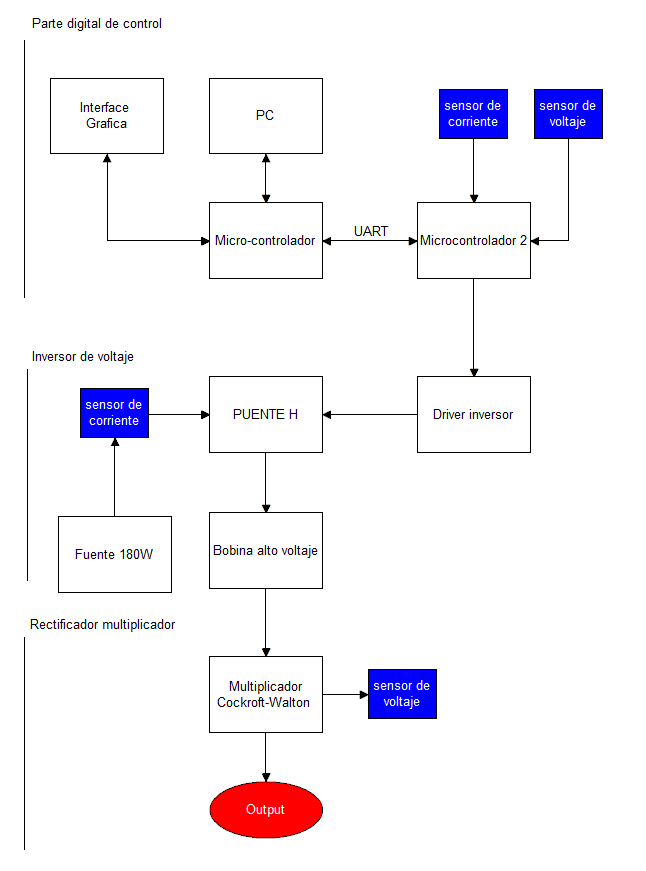
\includegraphics[width=12cm]{capitulo2/figs/figura1.png}
\caption{Calculo de ancho de pistas 1}
\end{figure}

\begin{figure}[H]
\centering
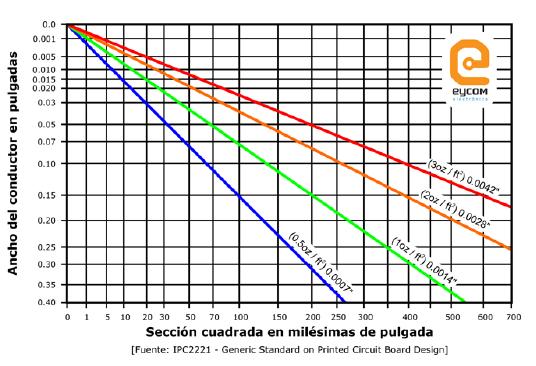
\includegraphics[width=12cm]{capitulo2/figs/figura2.png}
\caption{Calculo de ancho de pistas 1}
\end{figure}

\newpage
\section{Fuente de voltaje lineal}
Es común en proyectos de electrónica no especializados la utilización de diferentes tipos de fuentes de voltaje, entre las que se encuentran fuentes lineales, conmutadas, boost o tipo buck y los problemas que puede causar la falta de atención en este punto tan crucial puede afectan los resultados finales de un proyecto. Es por ello que se necesita conocer los principios fundamentales que reinan a este tipo de sistemas que gobernaran el comportamiento de nuestro proyecto al nivel mas básico.\\

La fuente de voltaje lineal consiste en un sistema sencillo y estructurado, el cual se diseña en diferentes configuraciones en cada modulo a partir del tipo de carga que requiere el proyecto. Para ello podemos observar en la figura 2.5 de manera ilustrativa el orden de la estructura básica de una fuente lineal.

\begin{figure}[H]
 \centering
 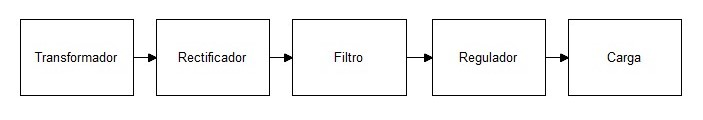
\includegraphics[width=12cm]{capitulo2/figs/fuentelineal.jpg}
 \caption{estructura fuente lineal}
 \end{figure}
 
 De manera independiente podemos analizar cada aspecto presentado en la imagen, el cual, de uno en uno se va realizando un análisis para definir los valores y topologias que satisfacen las necesidades requeridas. Tomando en cuenta lo mencionado podemos comenzar a definir las ecuaciones y modelos existentes.

\newpage

\section{Inversores de voltaje}

\section{Bobina de ignición}
das
\section{Fuentes de alto voltaje mas comunes}


\section{Multiplicador de voltaje Cockcroft-Walton}
fgdgf           % ~20 páginas - Poner un contexto a la tesis, hacer referencia a trabajos actuales en el tema

%%%%%%%%%%%%%%%%%%%%%%%%%%%%%%%%%%%%%%%%%%%%%%%%%%%%%%%%%%%%%%%%%%%%%%%%%
%           Capítulo 3: Metodologia                   %
%%%%%%%%%%%%%%%%%%%%%%%%%%%%%%%%%%%%%%%%%%%%%%%%%%%%%%%%%%%%%%%%%%%%%%%%%

\chapter{Metodología}
En este capítulo se expone todo el desarrollo de la fuente de alto voltaje en cuestión; diseño del sistema, fabricación del sistema, diseño del firmware del micro controlador, implementación y por último el método experimental.\\

El sistema esta compuesto por dos partes, hardware y firmware, el hardware se compone de tres partes como vemos en la figura 3.1: parte digital de control, inversor de voltaje y rectificador multiplicador. \\

Por otro lado el firmware consiste en los programas que realizan el control completo de la generación de alto voltaje por medio del desarrollo de un ambiente gráfico al que el usuario tiene acceso,  control para el senseo de voltajes, corrientes y protecciones necesarias para el correcto funcionamiento del sistema en general, así como también un control para el inversor de voltaje, mediante la implementación de un ADC ( Analog to Digital Converter) a la salida de una devanado de baja en el transformador de alto voltaje el cual controla la salida de alto voltaje. Observemos de manera gráfica la topologia del sistema en la figura 3.1. 



 % The \cite command functions as follows:
 %   \citet{key} ==>>                Jones et al. (1990)
 %   \citet*{key} ==>>               Jones, Baker, and Smith (1990)
 %   \citep{key} ==>>                (Jones et al., 1990)
 %   \citep*{key} ==>>               (Jones, Baker, and Smith, 1990)
 %   \citep[chap. 2]{key} ==>>       (Jones et al., 1990, chap. 2)
 %   \citep[e.g.][]{key} ==>>        (e.g. Jones et al., 1990)
 %   \citep[e.g.][p. 32]{key} ==>>   (e.g. Jones et al., p. 32)
 %   \citeauthor{key} ==>>           Jones et al.
 %   \citeauthor*{key} ==>>          Jones, Baker, and Smith
 %   \citeyear{key} ==>>             1990





%%%%%%%%%%%%%%%%%%%%%%%%%%%%%%%%%%%%%%%%%%%%%%%%%%%%%%%%%%%%%%%%%%%%%%%%%
%                          Descripción de la planta                     %
%%%%%%%%%%%%%%%%%%%%%%%%%%%%%%%%%%%%%%%%%%%%%%%%%%%%%%%%%%%%%%%%%%%%%%%%%
\section{Diseño del hardware}


La figura 3.1 muestra un diagrama a bloques de la estructura general del hardware que conforma el sistema de generación de alto voltaje, el cual esta compuesto, desde la parte superior a la inferior, primeramente por bloques relacionados con el control digital del sistema, este bloque se encarga de las interfaces para el usuario así como también de el control e instrumentación de los diferentes sensores, el siguiente conjunto de bloques representan la electrónica encargada de la inversión de voltaje y por ultimo tenemos la rectificación.  \\

\begin{figure}[H]
\centering
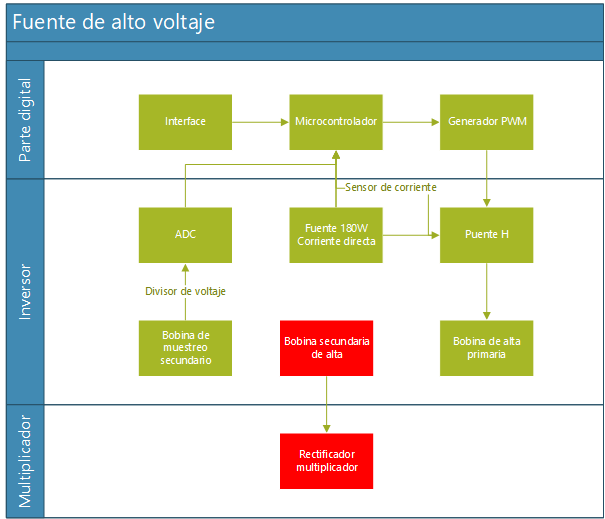
\includegraphics[width=12
cm]{Capitulo3/figs/diagrama.png}
\caption{Topologia de fuente de alto voltaje}
\end{figure}
\subsection{Hardware de interface}
Para el desarrollo de la interface gráfica se a utilizado un microcontrolador ATMEGA2560, implementado por la facilidad de programación y los tiempos cortos para la conclusión de este proyecto, así como también la implementación de una pantalla TFT-LCD ( Pantalla de cristal líquido de transistores de película fina) y comunicación UART como interfaces gráfica al usuario. Se ha utilizado el hardware de dicha placa y ahorrado tiempo de desarrollo. \\


\begin{figure}[H]
\centering
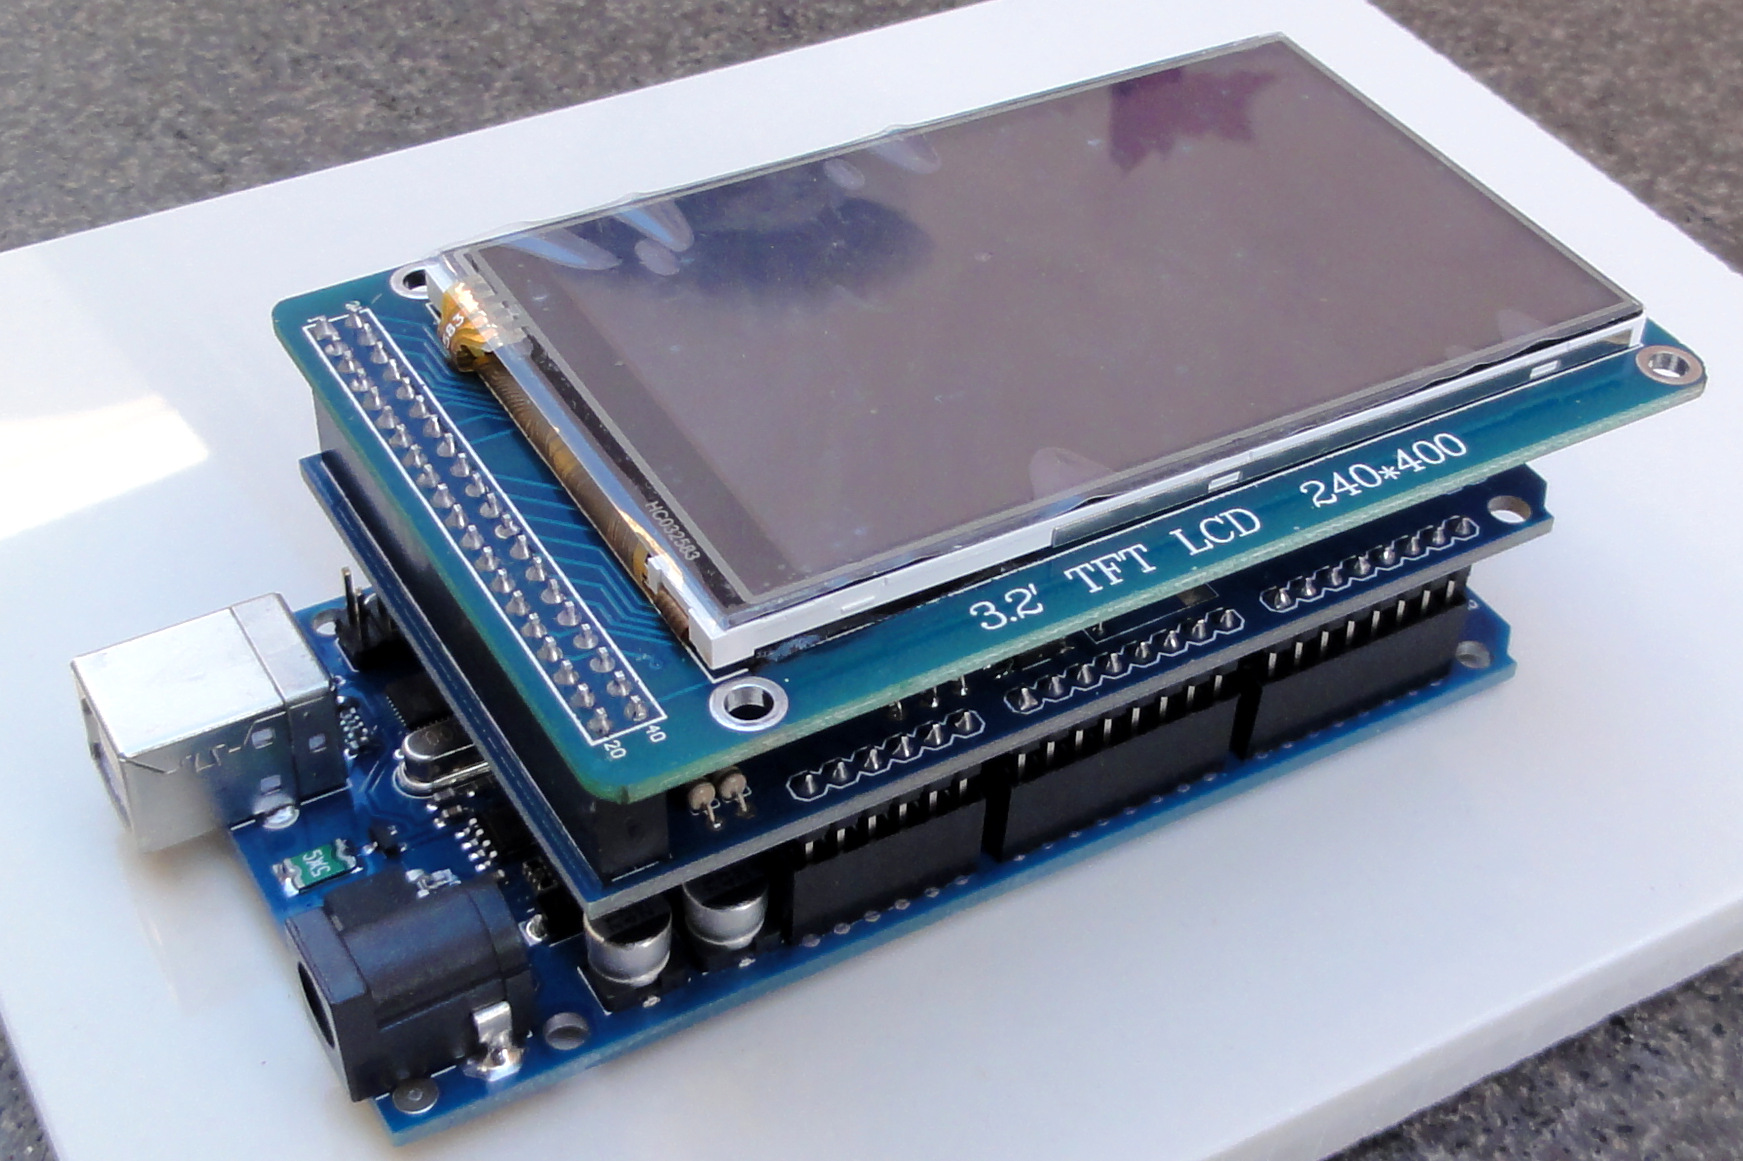
\includegraphics[width=9
cm]{Capitulo3/figs/pantalla0.jpg}
\caption{LCD-TFT para interface gráfica}
\end{figure}
\subsection{Hardware de fuente de voltaje 180w}

Esta sección consiste en varias etapas de desarrollo, para ello primero se ha desarrollado una fuente de voltaje de 180W, que es el primer circuito a analizar. Podemos observar en la figura 3.2 el diseño propuesto. El cual esta conformado por el regulador de voltaje LM723 en modalidad fuente de voltaje por modalidad de regulación positiva.

\begin{figure}[H]
\centering
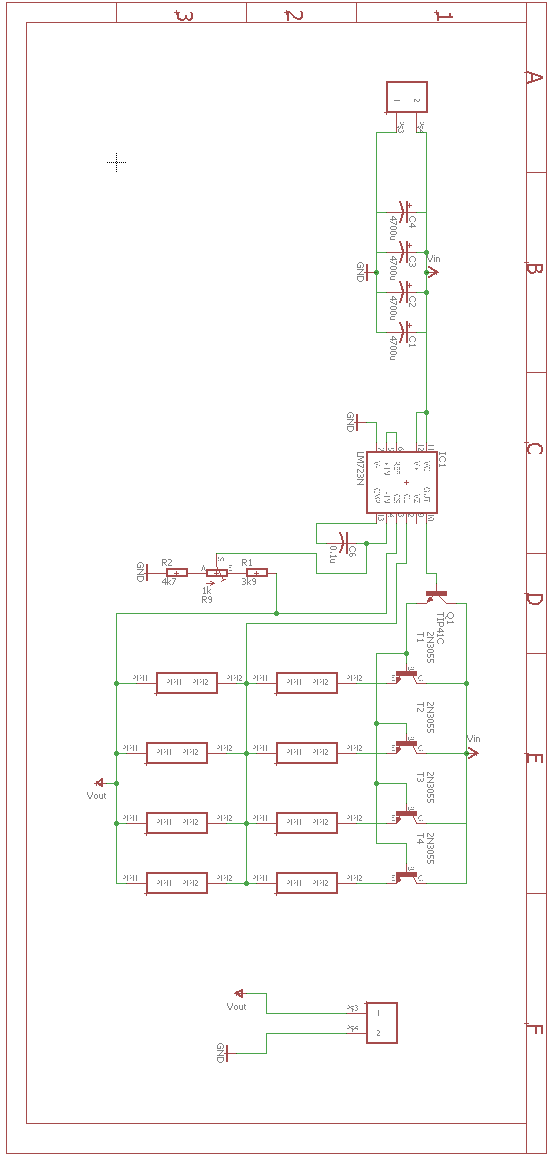
\includegraphics[width=10cm]{Capitulo3/figs/fuente.png}
\caption{Topologia de fuente de alto voltaje}
\end{figure}

Se ha simulado esta fuente de voltaje en el programa LTSPICE como se muestra en la figura 3.4 con la finalidad de encontrar el voltaje RMS teórico en nuestra salida con diferentes cargas, ya que se busca el menor riso posible en nuestra salida final, ya que, en este punto el ruido sera amplificado cientos de veces. \\
\begin{figure}[H]
\centering
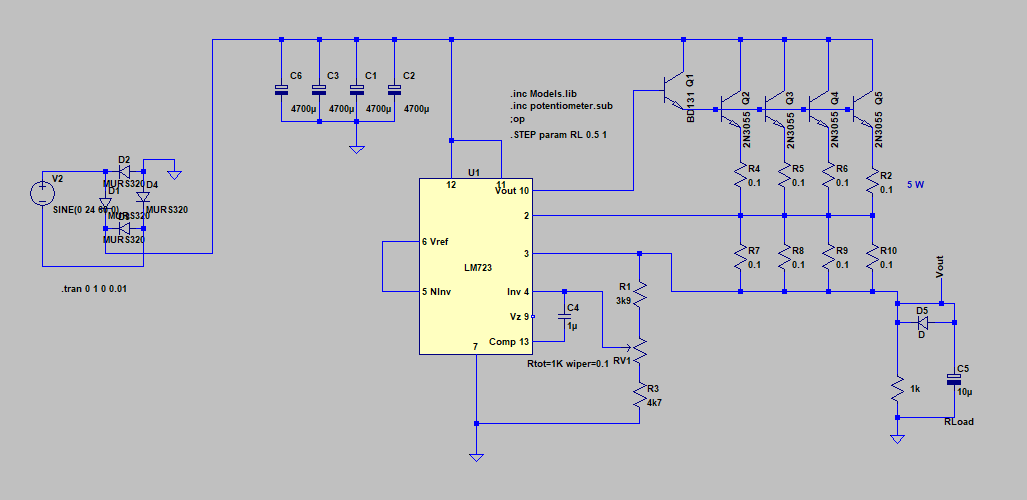
\includegraphics[width=12cm]{Capitulo3/figs/SIMFUENTE.png}
\caption{Simulación en LTSPICE fuente 180w}
\end{figure}
Mediante ROOT CERN se ha creado una distribución gaussiana del voltaje RMS para tres cargas diferentes, sin carga, a 9.6W y a 19.2w mediante estas mediciones podemos calcular la eficiencia de nuestra fuente de voltaje con la ecuacion XXX.\\

[Poner aquí las ecuaciones y evaluarlas con los resultados de las simulaciones y de las mediciones]

\begin{figure}[H]
\centering
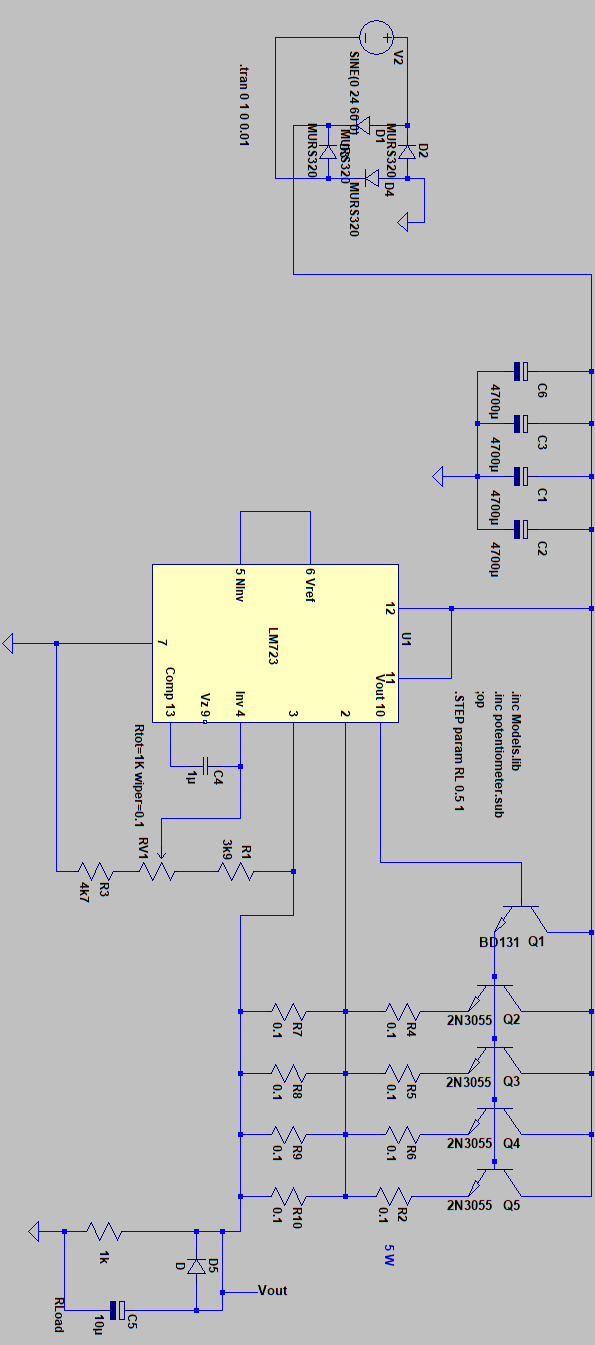
\includegraphics[width=8cm]{Capitulo3/figs/sim.png}
\caption{Topologia de fuente de alto voltaje}
\end{figure}


\section{Firmware}
\subsection{Interface gráfica}
Para el desarrollo de la interface grafica se ha realizado en el ambiente de programación de Arduino, intentando la utilizacion de la menor cantidad de librerias de autoria no propia y siguiendo algunas reglas de programacion basicas para micro-controladores como lo es la no utilizacion de los comandos delay. Dicho código se divide en varias secciones, para el cual solo se utilizaron las siguientes librerías:

\begin{verbatim}

#include <UTFT.h>
#include <URTouch.h>

\end{verbatim}

En la siguiente figura podemos observar la topologia del firmware que se ha desarrollado.\\

Todo el código esta dividido en funciones, las cuales llamamos en nuestro LOOP, tratando siempre de cumplir con las siguientes características: no utilización de la función delay, no utilización de ciclos que dependa de alguna condición externa, utilizar el menor código posible para una acción. Las funciones que se utilizaron para la el despliegue de información de la primera pantalla fue el siguiente:


\begin{verbatim}

 
void botones1(){ 
  myGLCD.setFont(BigFont); 
  for (x=0; x<3; x++)
  {
    myGLCD.setColor(0, 0, 255);
    myGLCD.fillRoundRect (200, 10+(x*55), 310, 60+(x*55));
    myGLCD.setColor(255, 255, 255);
    myGLCD.drawRoundRect (200, 10+(x*55), 310, 60+(x*55));
  }
for (x=0; x<2; x++)
  {
    myGLCD.setColor(0, 0, 255);
    myGLCD.fillRoundRect (10+(x*155), 175, 155+(x*155), 225);
    myGLCD.setColor(255, 255, 255);
    myGLCD.drawRoundRect (10+(x*155), 175, 155+(x*155), 225);
  }
  myGLCD.setBackColor(0, 0, 255);
  myGLCD.print("ON 2", 220 , 30);
  myGLCD.print("ON 3", 220 , 85);
  myGLCD.print("ON 1", 220 , 140);
  //myGLCD.print("UART ON", 185 , 195);
  myGLCD.print("V SET", 40 , 190);
  myGLCD.print("CONFIG", 190 , 190);
  }
  
void marco1(int x1, int y1, int x2, int y2){ 
  myGLCD.setColor(255, 0, 0);
  myGLCD.drawRoundRect (x1, y1, x2, y2);
  while (myTouch.dataAvailable())
  myTouch.read();
  myGLCD.setColor(255, 255, 255);
  myGLCD.drawRoundRect (x1, y1, x2, y2);
}
\end{verbatim}

Mediante el código anterior podemos, con ciertas variables, dibujar nuestra área de trabajo en la pantalla, obteniendo como resultado el dibujo de la figura XXX.

\begin{figure}[H]
\centering
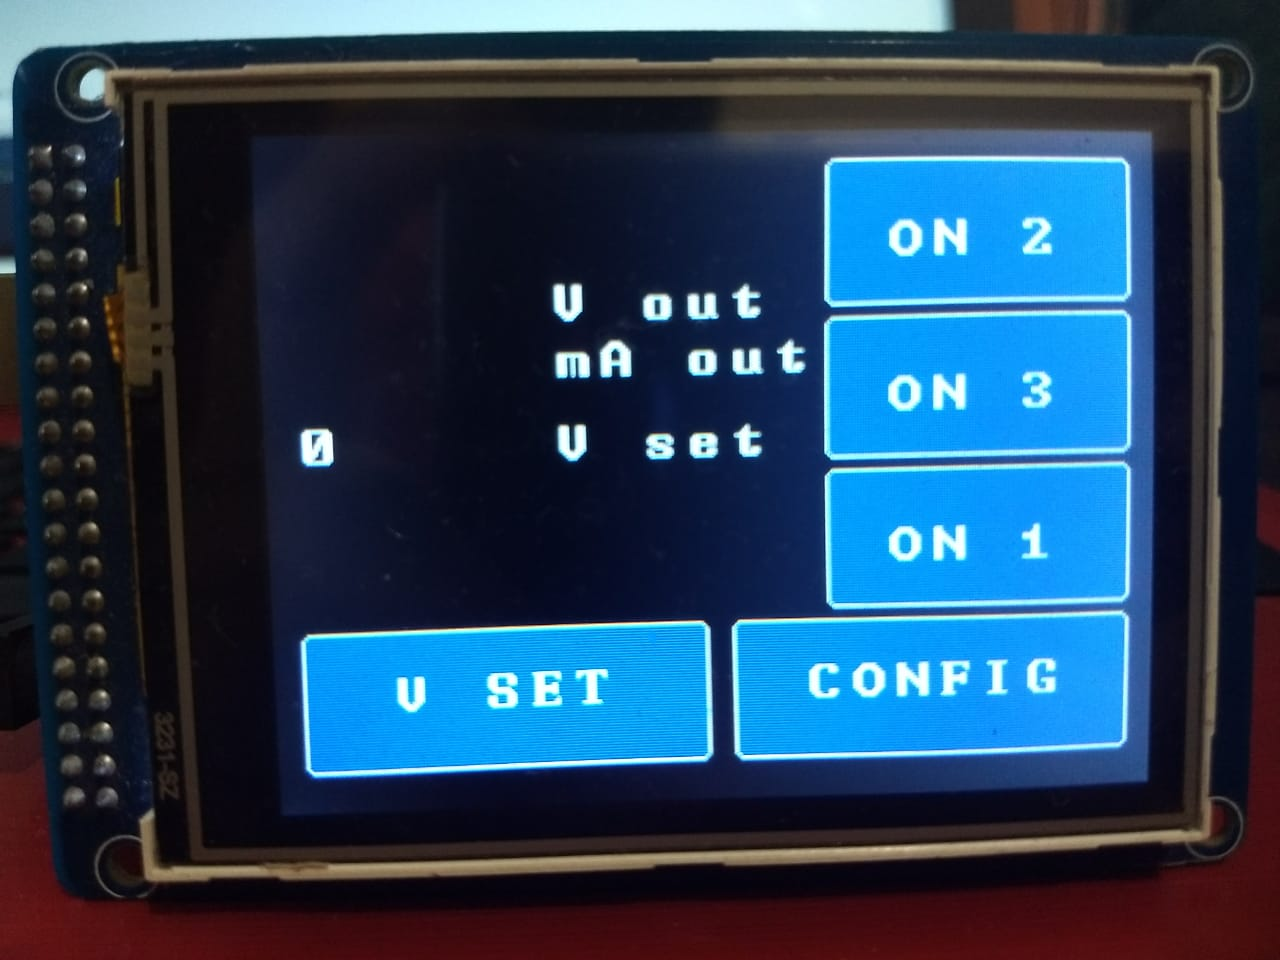
\includegraphics[width=8cm]{Capitulo3/figs/pantalla1.jpg}
\caption{Pantalla 1}
\end{figure}

Mediante esta configuración de dibujo partimos para el código de configuración del TOUCH para lo que llamamos la "pantalla 1".

\begin{verbatim}
void touch1(){ 
      myTouch.read();
      x=myTouch.getX();
      y=myTouch.getY();
      if((x>=200) && (x<=310))
      {
        if((y>=10) && (y<=60)){ //boton ON 2
          marco1(200,10,310,60);
        }
        if((y>=65) && (y<=115)){ //boton ON 3
          marco1(200,65,310,115);
        }
        if((y>=120) && (y<=170)){ //boton ON 1
          marco1(200,120,310,170);
        }
      }
      if((y>=175) && (y<=225))
      {
        if((x>=10) && (x<=155)){ //boton V SET
          marco1(10,175,155,225);
          pantalla =2;
        }
      
        if((x>=165) && (x<=310)){ //boton config
          marco1(165,175,310,225);
        }
}
}
\end{verbatim}

Observamos que el despliegue de estas funciones solo están conformadas por elementos "if" y el llamado a funciones descritas por nosotros se despliegan de la misma manera, resaltando esto debido a que se desarrollo un código lo mas eficientemente posible en cuestión de tiempos de ejecución. \\

Dividimos el dibujo de la "pantalla 2" y las funciones para el touch de la pantalla dos en los siguientes codigos:\\

Funciones dibujo pantalla 2

\begin{verbatim}
void botones2(){
  myGLCD.setBackColor(0,0,255);
  for (x=0; x<4; x++) //botones +
  {
    myGLCD.setColor(0, 0, 255);
    myGLCD.fillRoundRect (10+(x*60), 10, 60+(x*60), 60);
    myGLCD.setColor(255, 255, 255);
    myGLCD.drawRoundRect (10+(x*60), 10, 60+(x*60), 60);
    myGLCD.print("+", 27+(x*60), 27);
  }


  for (x=0; x<4; x++) //botones -
  {
    myGLCD.setColor(0, 0, 255);
    myGLCD.fillRoundRect (10+(x*60), 170, 60+(x*60), 220);
    myGLCD.setColor(255, 255, 255);
    myGLCD.drawRoundRect (10+(x*60), 170, 60+(x*60), 220);
    myGLCD.print("-", 27+(x*60), 190);
  }

  for (x=0; x<4; x++) //blanco 
  {
    myGLCD.setColor(255, 255, 255);
    myGLCD.fillRoundRect (10+(x*60), 70, 60+(x*60), 160);
    myGLCD.setColor(255, 0, 0);
    myGLCD.drawRoundRect (10+(x*60), 70, 60+(x*60), 160);
  //  myGLCD.print(p, 27+(x*60), 170);
  }

  myGLCD.setColor(0, 0, 255); /// boton set
   myGLCD.fillRoundRect(250,70,310,160);
   myGLCD.setColor(255, 255, 255);
   myGLCD.drawRoundRect(250,70,310,160);
   myGLCD.print("set" , 255,105);
  }
\end{verbatim}

Podemos observar el resultado del dibujo en la figura XXX.

\begin{figure}[H]
\centering
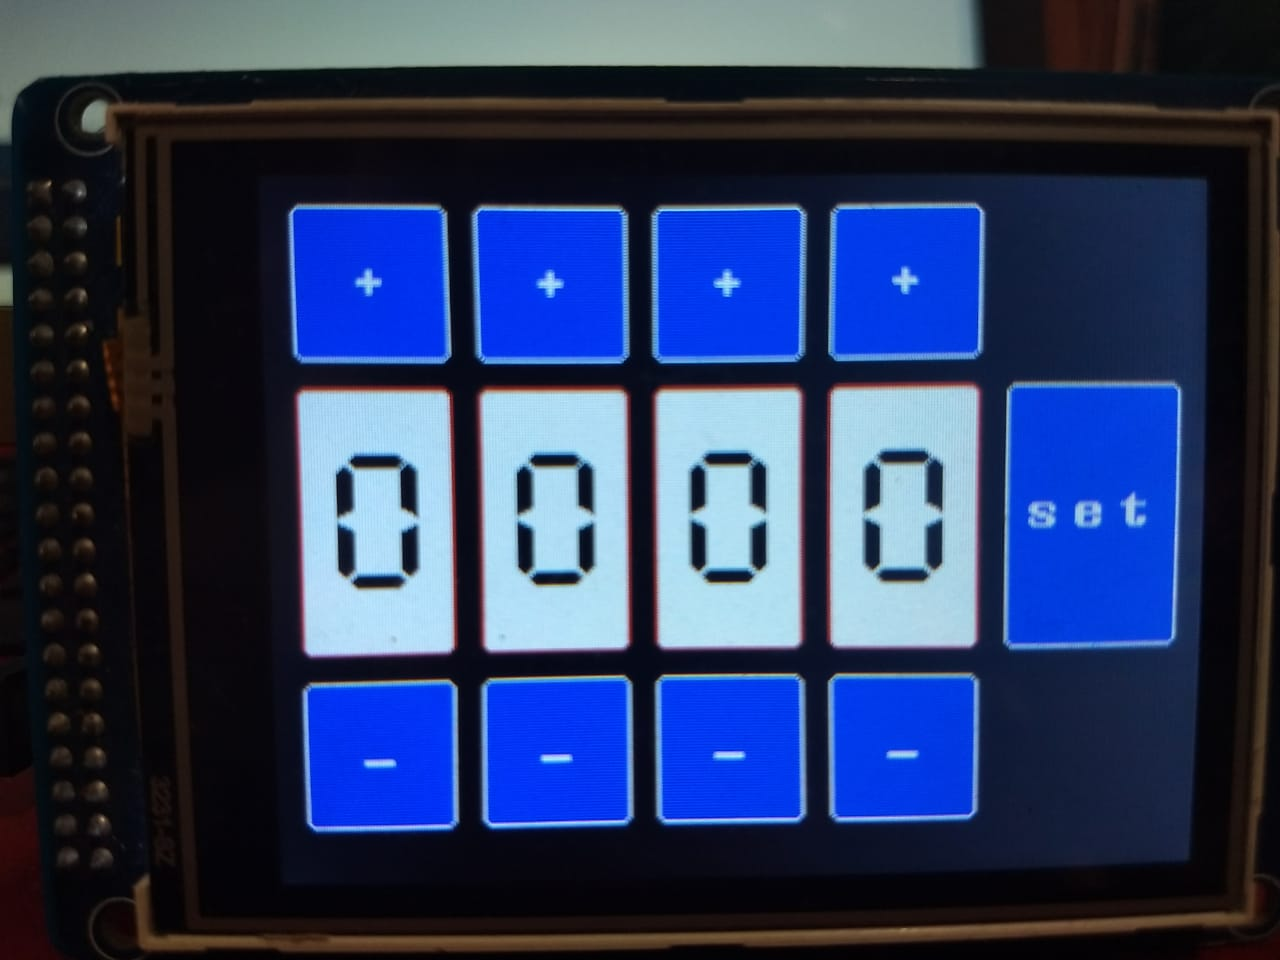
\includegraphics[width=8cm]{Capitulo3/figs/pantalla2.jpg}
\caption{Pantalla 2}
\end{figure}

 Funciones TOUCH pantalla 2:
\begin{verbatim}
void touch2(){
    myTouch.read();
      x=myTouch.getX();
      y=myTouch.getY();

      if((y>=10) && (y<=60)){ /////////////botones +
        if((x>=10) && (x<=60)){ //boton + kilos
          marco1(10,10,60,60);
          
          myGLCD.setFont(SevenSegNumFont); 
          suma(1,0,0,0,0,0);
        }

        if((x>=70) && (x<=120)){ //boton + centena
          marco1(70,10,120,60);
          suma(0,1,0,0,0,0);
          
          
        }

        if((x>=130) && (x<=180)){ //boton + decena
          marco1(130,10,180,60); 
          suma(0,0,1,0,0,0);
          
        }

        if((x>=190) && (x<=240)){ //boton + unidad
          marco1(190,10,240,60);
          suma(0,0,0,1,0,0);
          
        }
        }
        if((y>=170) && (y<=220)){ ////////////botones -
          
        if((x>=10) && (x<=60)){ //boton + kilos
          marco1(10,170,60,220);
          suma(1,0,0,0,0,1);
        }

        if((x>=70) && (x<=120)){ //boton + centena
          marco1(70,170,120,220);
          suma(0,1,0,0,0,1);
        }

        if((x>=130) && (x<=180)){ //boton + decena
          marco1(130,170,180,220);
          suma(0,0,1,0,0,1);
        }

        if((x>=190) && (x<=240)){ //boton + unidad
          marco1(190,170,240,220);
          suma(0,0,0,1,0,1);
        }
        }

        if((x>=250) && (x<=310)){ // boton SET

          if((y>=70) && (y<=160)){
            marco1(250,70,310,160);
            pantalla =1;
            if(vout >=0 && vout <=1000){
            Serial.println(vout);
            }
            }    
        }
    }
\end{verbatim}

Una vez que definimos las funciones a utilizar para estas dos primeras pantallas proseguimos a las funciones de cálculos y procesamiento de datos. Para ello hemos creado una funcion capaz de configurar el voltaje de salida, manteniendo una comunicación UART hacia un micro-controlador. 

\begin{verbatim}
void suma(int x1,int x2,int x3,int x4, int k, int w){ 
          myGLCD.setFont(SevenSegNumFont);
          myGLCD.setColor(0, 0, 0);
          myGLCD.setBackColor(255,255,255);
          int q;  
          if(x1 == 1){//algoritmo kilos
            if(w==0 && p<9){
            vout=vout+1000;
            p=p+1;
            q=p*x1+p1*x2+p2*x3+p3*x4;
            sprintf(dato,"%d",q);
            }
            if(w==1 && p>0){
            vout=vout-1000;
            p=p-1;
            q=p*x1+p1*x2+p2*x3+p3*x4;
            sprintf(dato,"%d",q);
              
              }
            myGLCD.print(dato,20*x1+80*x2+140*x3+200*x4,90);
          }
          if(x2 == 1){//algoritmo centena
            if(w==0 && p1<9){
            vout=vout+100;
            p1=p1+1;
            q=p*x1+p1*x2+p2*x3+p3*x4;
            sprintf(dato,"%d",q);
            }
            if(w==1 && p1>0){
            vout=vout-100;
            p1=p1-1;
            q=p*x1+p1*x2+p2*x3+p3*x4;
            sprintf(dato,"%d",q);
              
              }
            myGLCD.print(dato,20*x1+80*x2+140*x3+200*x4,90);
          }
          if(x3 == 1){//algoritmo decenas
            if(w==0 && p2<9){
            vout=vout+10;
            p2=p2+1;
            q=p*x1+p1*x2+p2*x3+p3*x4;
            sprintf(dato,"%d",q);
            }
            if(w==1 && p2>0){
            vout=vout-10;
            p2=p2-1;
            q=p*x1+p1*x2+p2*x3+p3*x4;
            sprintf(dato,"%d",q);
              
              }
            myGLCD.print(dato,20*x1+80*x2+140*x3+200*x4,90);
            //Serial.println(vout);
          }
          if(x4 == 1){//algoritmo unidades
            if(w==0 && p3<9){
            vout=vout+1;
            p3=p3+1;
            q=p*x1+p1*x2+p2*x3+p3*x4;
            sprintf(dato,"%d",q);
            }
            if(w==1 && p3>0){
            vout=vout-1;
            p3=p3-1;
            q=p*x1+p1*x2+p2*x3+p3*x4;
            sprintf(dato,"%d",q);
              
              }
            myGLCD.print(dato,20*x1+80*x2+140*x3+200*x4,90);
          }
          
          if(k==1){
            for(x=0 ; x<4 ; x++){
              sprintf(dato,"%d",p);
              myGLCD.print(dato,20,90);
              sprintf(dato,"%d",p1);
              myGLCD.print(dato,80,90);
              sprintf(dato,"%d",p2);
              myGLCD.print(dato,140,90);
              sprintf(dato,"%d",p3);
              myGLCD.print(dato,200,90);
              }
            }
    }
\end{verbatim}

Una segunda funcion es la encargada de recibir los datos procedentes del segundo micro-controlador, encargado de leer los datos de sensores y preparar el funcionamiento del inversor. 

\begin{verbatim}
void vinput(){
  
      str = Serial.readStringUntil('\n');
      for (int i = 0; i < dataLength ; i++)
      {
         int index = str.indexOf(separator);
         data[i] = str.substring(0, index).toInt();
         str = str.substring(index + 1);
      }
      
      for (int i = 0; i < sizeof(data) / sizeof(data[0]); i++)    
      {
        Serial.print(data[i]); 
      Serial.print('\t');} 
      Serial.println();
      
                  myGLCD.setFont(BigFont);
                  sprintf(vin, "%d",data[0]);
                  sprintf(current, "%d", data[1]);
                  myGLCD.print("     " ,10,50);
                  myGLCD.print("     " ,10,70);
                  myGLCD.setBackColor(0,0,0);
                  myGLCD.setColor(255,255,255);
                  myGLCD.print(vin ,10,50);
                  myGLCD.print(current ,10,70);
  }
\end{verbatim}

Mediante las funciones anteriores podemos mantener una comunicacion INPUT y OUTPUT mediante UART, con el segundo micro-controlador, y mantener un senseo de las variables necesarias para el correcto funcionamiento de la fuente de alto voltaje. Ahora mostramos en cuerpo del programa principal, encargado del control de cada una de las funciones anteriores.

\begin{verbatim}
void loop(){

//pantalla 1
if(pantalla == 1){
    myGLCD.fillScr(VGA_BLACK);
    botones1();
    myGLCD.setFont(BigFont); 
    char set[25];
    sprintf(set, "%d",vout);
    myGLCD.setBackColor(0,0,0);
    myGLCD.print(set ,10,100);
    myGLCD.print("V set" ,100,100);
    myGLCD.print("V out" ,100,50);
    myGLCD.print("mA out" ,100,70);
    myGLCD.print(vin ,10,50);
    myGLCD.print(current ,10,70);
    while(true)
         {
          if(myTouch.dataAvailable())touch1();
          if(pantalla == 2 )break;

      if (Serial.available()>0){vinput();}
            }
            }
          
        
//pantalla 2
if(pantalla == 2){
  myGLCD.fillScr(VGA_BLACK);
  
  botones2();
  
  suma(0,0,0,0,1,0);
  while(true)
    {
      if(myTouch.dataAvailable())touch2();
      if(pantalla == 1)break;
    }
  }


  }
\end{verbatim}      % ~20 páginas - Explicar el problema en específico que se va a resolver, la metodología y experimentos/métodos utilizados
\chapter{Análisis de Resultados}
\section{Resultados}

Se ha logrado mediante la implementación de un sistema de inversor de voltaje alcanzar voltajes de hasta 2 KV a una potencia de 40w, voltaje controlado digitalmente por un computador. Se ha desarrollado un código en root CERN para encontrar el voltaje RMS de nuestro voltaje de salida. Nuestras mediciones realizadas arrojaron las siguientes distribuciones para diferentes voltajes sin carga alguna. \\

\begin{figure}[H]
\centering
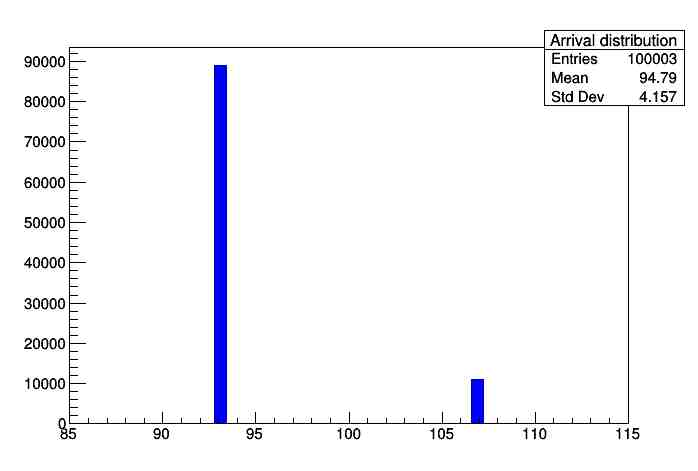
\includegraphics[width=12cm]{Capitulo4/93v.jpg}
\caption{Salida alto voltaje sin carga a 93v.}
\end{figure}

\begin{figure}[H]
\centering
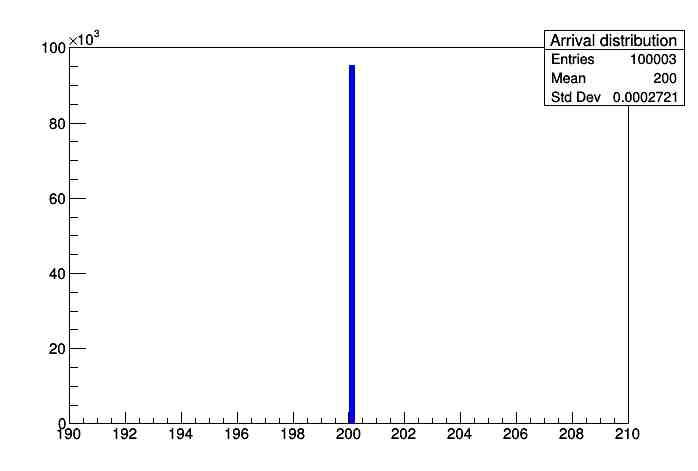
\includegraphics[width=12cm]{Capitulo4/200v.jpg}
\caption{Salida alto voltaje sin carga a 200v.}
\end{figure}

\begin{figure}[H]
\centering
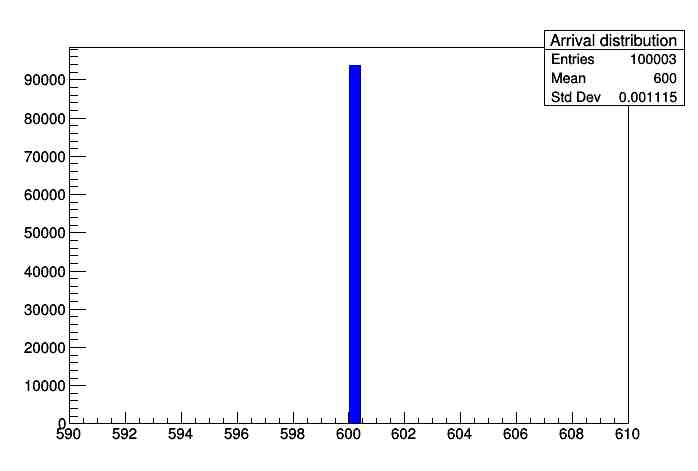
\includegraphics[width=12cm]{Capitulo4/600v.jpg}
\caption{Salida alto voltaje sin carga a 600v.}
\end{figure}

\begin{figure}[H]
\centering
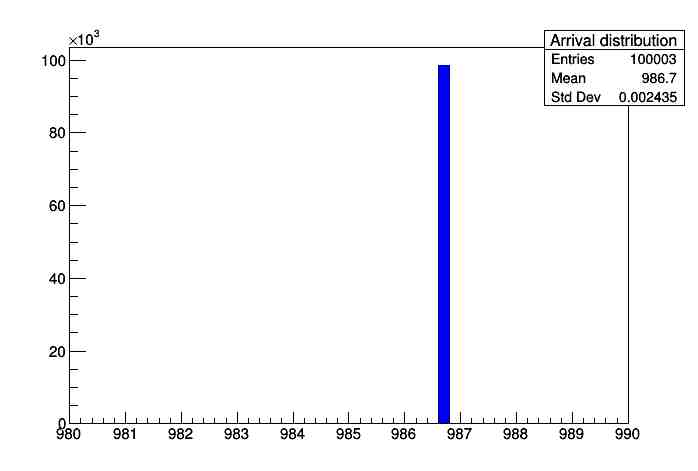
\includegraphics[width=12cm]{Capitulo4/986v.jpg}
\caption{Salida alto voltaje sin carga a 986v.}
\end{figure}
\newpage

Como observamos se ha obtenido voltajes sin perturbaciones y con relativo bajo rizo asociado a él. Se realizaron diez mil mediciones por cada distribución y a partir de ella podemos observar un voltaje RMS de 4.15v a 93v, 0.00027v para 200v, 0.0011v para 600v y 0.0024v para 986v respectivamente. \\

Utilizando la ecuación 2.6 podemos calcular el rizo asociado a la señal. Se observa en la tabla los siguientes resultados de nuestras mediciones con sus variables correspondientes. 

\begin{table}[H]
\begin{tabular}{@{}llll@{}}
\toprule
Voltaje   & Frecuencia & Dutty & Riso \\ \midrule
93  & o.o        & 0.0   &  0.0\\
200 & 0.0        & 0.0   &   0.0\\
600 & 0.0        & 0.0   &   0.0\\
986 & 0.0        & 0.0   &   0.0\\ \bottomrule
\end{tabular}
\end{table}


Los resultados indican que se ha desarrollado una fuente con requerimientos suficientes para trabajos de laboratorio.    % ~20 páginas - Presentar los resultados tal cual son, y analizarlos.
\chapter{Conclusiones}
Se logro la construcción satisfactoria de una fuente de alto voltaje controlada digitalmente mediante un computador y de forma manual mediante un microcontrolador integrado. Los voltajes máximos alcanzados fueron mas de 3.8KV, limitados por nuestros instrumentos de medición. Con una potencia de hasta 20W y un rizo bastante bajo.\\

La caída de voltaje es el valor que representa el mayor problema en nuestro circuito, siendo necesario el desarrollo de una retroalimentación que ajuste el voltaje en tiempo real, reduciendo así dicha caída. Nuestro inversor y fuente de voltaje de CD fueron diseñados para soportar hasta 180W, así como también nuestro transformador de alto voltaje, por lo que el ajuste en potencia de esta retroalimentación se puede realizar digitalmente como futura continuación del proyecto.            % ~5 páginas - Resumir lo que se hizo y lo que no y comentar trabajos futuros sobre el tema

\end{large}
%%%%%%%%%%%%%%%%%%%%%%%%%%%%%%%%%%%%%%%%%%%%%%%%%%%%%
%                   APÉNDICES                       %
%%%%%%%%%%%%%%%%%%%%%%%%%%%%%%%%%%%%%%%%%%%%%%%%%%%%%
\appendix
% this file is called up by thesis.tex
% content in this file will be fed into the main document
\chapter{Código/Manuales/Publicaciones}
\section{Código pantalla táctil}
\begin{verbatim}

/////////////////////////////////////
//programa para control de alto voltaje
//mediante la implementacion de LCD TOUCH TFT de 3.2
//
//
//
/////////////////////////////////////
#include <UTFT.h>
#include <URTouch.h>



//indicamos pines para hardware
UTFT    myGLCD(ILI9341_16,38,39,40,41);
URTouch  myTouch( 6, 5, 4, 3, 2);


//Definimos fuentes que utilizaremos
extern uint8_t SmallFont[];
extern uint8_t BigFont[];
extern uint8_t SevenSegNumFont[];

//variables que estaremos utilizando
int x,y,pantalla=1,k,voltaje=1,p=0,p1=0,p2=0,p3=0,vout=0;
char dato[20];

//variables para tomar datos de UART

String str = "";
const char separator = ',';
const int dataLength = 2;
int data[dataLength];
char vin[20];
      char current[20];


void botones1(){ ///////////////////////////////////////botones pantalla 1
  myGLCD.setFont(BigFont); 

  for (x=0; x<3; x++)
  {
    myGLCD.setColor(0, 0, 255);
    myGLCD.fillRoundRect (200, 10+(x*55), 310, 60+(x*55));
    myGLCD.setColor(255, 255, 255);
    myGLCD.drawRoundRect (200, 10+(x*55), 310, 60+(x*55));
    
  }

for (x=0; x<2; x++)
  {
    myGLCD.setColor(0, 0, 255);
    myGLCD.fillRoundRect (10+(x*155), 175, 155+(x*155), 225);
    myGLCD.setColor(255, 255, 255);
    myGLCD.drawRoundRect (10+(x*155), 175, 155+(x*155), 225);
    
  }



  
  myGLCD.setBackColor(0, 0, 255);
  myGLCD.print("ON 2", 220 , 30);
  myGLCD.print("ON 3", 220 , 85);
  myGLCD.print("ON 1", 220 , 140);
  //myGLCD.print("UART ON", 185 , 195);
  myGLCD.print("V SET", 40 , 190);
  myGLCD.print("CONFIG", 190 , 190);
  
  
  
  }
  
  
  
void marco1(int x1, int y1, int x2, int y2){ //////////////////////////marcos pantalla 1
  myGLCD.setColor(255, 0, 0);
  myGLCD.drawRoundRect (x1, y1, x2, y2);
  while (myTouch.dataAvailable())
  myTouch.read();
  myGLCD.setColor(255, 255, 255);
  myGLCD.drawRoundRect (x1, y1, x2, y2);
  
}

void touch1(){ ///////////////////////////////////////////////////////funciones de touch pantalla 1
  
      myTouch.read();
      x=myTouch.getX();
      y=myTouch.getY();

      if((x>=200) && (x<=310))
      {
        if((y>=10) && (y<=60)){ //boton ON 2
          marco1(200,10,310,60);
        }
        
        if((y>=65) && (y<=115)){ //boton ON 3
          marco1(200,65,310,115);

        }

        if((y>=120) && (y<=170)){ //boton ON 1
          marco1(200,120,310,170);
   
        }

       
      }

      if((y>=175) && (y<=225))
      {
        if((x>=10) && (x<=155)){ //boton V SET
          marco1(10,175,155,225);
          pantalla =2;
        }
      
        if((x>=165) && (x<=310)){ //boton config
          marco1(165,175,310,225);
          
        }
}
}

////////////////////////////// fin de pantalla 1


//////////////////////////////////////////////////////////////////////////// pantalla 2

void botones2(){ /////////////////////////////////////////////////////////// botones pantalla 2
  myGLCD.setBackColor(0,0,255);
  for (x=0; x<4; x++) //botones +
  {
    myGLCD.setColor(0, 0, 255);
    myGLCD.fillRoundRect (10+(x*60), 10, 60+(x*60), 60);
    myGLCD.setColor(255, 255, 255);
    myGLCD.drawRoundRect (10+(x*60), 10, 60+(x*60), 60);
    myGLCD.print("+", 27+(x*60), 27);
  }


  for (x=0; x<4; x++) //botones -
  {
    myGLCD.setColor(0, 0, 255);
    myGLCD.fillRoundRect (10+(x*60), 170, 60+(x*60), 220);
    myGLCD.setColor(255, 255, 255);
    myGLCD.drawRoundRect (10+(x*60), 170, 60+(x*60), 220);
    myGLCD.print("-", 27+(x*60), 190);
  }

  for (x=0; x<4; x++) //blanco 
  {
    myGLCD.setColor(255, 255, 255);
    myGLCD.fillRoundRect (10+(x*60), 70, 60+(x*60), 160);
    myGLCD.setColor(255, 0, 0);
    myGLCD.drawRoundRect (10+(x*60), 70, 60+(x*60), 160);
  //  myGLCD.print(p, 27+(x*60), 170);
  }

  myGLCD.setColor(0, 0, 255); /// boton set
   myGLCD.fillRoundRect(250,70,310,160);
   myGLCD.setColor(255, 255, 255);
   myGLCD.drawRoundRect(250,70,310,160);
   myGLCD.print("set" , 255,105);
  }

  void suma(int x1,int x2,int x3,int x4, int k, int w){ ///////////////////////algoritmo subir o bajar voltaje seteado
          myGLCD.setFont(SevenSegNumFont);
          myGLCD.setColor(0, 0, 0);
          myGLCD.setBackColor(255,255,255);
          int q;  
          if(x1 == 1){      //////////////////////////////////algoritmo kilos
            if(w==0 && p<9){
            vout=vout+1000;
            p=p+1;
            q=p*x1+p1*x2+p2*x3+p3*x4;
            sprintf(dato,"%d",q);
            }
            if(w==1 && p>0){
            vout=vout-1000;
            p=p-1;
            q=p*x1+p1*x2+p2*x3+p3*x4;
            sprintf(dato,"%d",q);
              
              }
            myGLCD.print(dato,20*x1+80*x2+140*x3+200*x4,90);
//            Serial.println(vout);
          }
          if(x2 == 1){ /////////////////////////////////////////algoritmo centena
            if(w==0 && p1<9){
            vout=vout+100;
            p1=p1+1;
            q=p*x1+p1*x2+p2*x3+p3*x4;
            sprintf(dato,"%d",q);
            }
            if(w==1 && p1>0){
            vout=vout-100;
            p1=p1-1;
            q=p*x1+p1*x2+p2*x3+p3*x4;
            sprintf(dato,"%d",q);
              
              }
            myGLCD.print(dato,20*x1+80*x2+140*x3+200*x4,90);
//            Serial.println(vout);
          }
          if(x3 == 1){ //////////////////////////////////////////algoritmo decenas
            if(w==0 && p2<9){
            vout=vout+10;
            p2=p2+1;
            q=p*x1+p1*x2+p2*x3+p3*x4;
            sprintf(dato,"%d",q);
            }
            if(w==1 && p2>0){
            vout=vout-10;
            p2=p2-1;
            q=p*x1+p1*x2+p2*x3+p3*x4;
            sprintf(dato,"%d",q);
              
              }
            myGLCD.print(dato,20*x1+80*x2+140*x3+200*x4,90);
            //Serial.println(vout);
          }
          if(x4 == 1){ ////////////////////////////////algoritmo unidades
            if(w==0 && p3<9){
            vout=vout+1;
            p3=p3+1;
            q=p*x1+p1*x2+p2*x3+p3*x4;
            sprintf(dato,"%d",q);
            }
            if(w==1 && p3>0){
            vout=vout-1;
            p3=p3-1;
            q=p*x1+p1*x2+p2*x3+p3*x4;
            sprintf(dato,"%d",q);
              
              }
            myGLCD.print(dato,20*x1+80*x2+140*x3+200*x4,90);
//            Serial.println(vout);
          }
          
           if(k==1){
            for(x=0 ; x<4 ; x++){
              sprintf(dato,"%d",p);
              myGLCD.print(dato,20,90);
              sprintf(dato,"%d",p1);
              myGLCD.print(dato,80,90);
              sprintf(dato,"%d",p2);
              myGLCD.print(dato,140,90);
              sprintf(dato,"%d",p3);
              myGLCD.print(dato,200,90);
              
              
              }
            
            }
    
    }
  
   void touch2(){ ////////////////////////////////////////////////////////touch pantalla 2
    myTouch.read();
      x=myTouch.getX();
      y=myTouch.getY();

      if((y>=10) && (y<=60)){ /////////////botones +
        if((x>=10) && (x<=60)){ //boton + kilos
          marco1(10,10,60,60);
          
          myGLCD.setFont(SevenSegNumFont); 
          suma(1,0,0,0,0,0);
         
          
        }

        if((x>=70) && (x<=120)){ //boton + centena
          marco1(70,10,120,60);
          suma(0,1,0,0,0,0);
          
          
        }

        if((x>=130) && (x<=180)){ //boton + decena
          marco1(130,10,180,60); 
          suma(0,0,1,0,0,0);
          
        }

        if((x>=190) && (x<=240)){ //boton + unidad
          marco1(190,10,240,60);
          suma(0,0,0,1,0,0);
          
        }
        }


        if((y>=170) && (y<=220)){ ////////////botones -
          
        if((x>=10) && (x<=60)){ //boton + kilos
          marco1(10,170,60,220);
          suma(1,0,0,0,0,1);
        }

        if((x>=70) && (x<=120)){ //boton + centena
          marco1(70,170,120,220);
          suma(0,1,0,0,0,1);
        }

        if((x>=130) && (x<=180)){ //boton + decena
          marco1(130,170,180,220);
          suma(0,0,1,0,0,1);
        }

        if((x>=190) && (x<=240)){ //boton + unidad
          marco1(190,170,240,220);
          suma(0,0,0,1,0,1);
        }
        }

        if((x>=250) && (x<=310)){ // boton SET

          if((y>=70) && (y<=160)){
            marco1(250,70,310,160);
            pantalla =1;
            if(vout >=0 && vout <=1000){
            Serial.println(vout);
            }
            }
          

        }
       
    
    }


///////////////////////fin pantalla set voltaje

void setup(){
  myGLCD.InitLCD();
  myGLCD.clrScr();
  myTouch.InitTouch();
  myTouch.setPrecision(PREC_HI);
  Serial.begin(9600);
  Serial.setTimeout(50);
  }
void vinput(){
  
      str = Serial.readStringUntil('\n');
      for (int i = 0; i < dataLength ; i++)
      {
         int index = str.indexOf(separator);
         data[i] = str.substring(0, index).toInt();
         str = str.substring(index + 1);
      }
      
      for (int i = 0; i < sizeof(data) / sizeof(data[0]); i++)    
      {
        Serial.print(data[i]); 
      Serial.print('\t');} 
      Serial.println();
      
                  myGLCD.setFont(BigFont);
                  sprintf(vin, "%d",data[0]);
                  sprintf(current, "%d", data[1]);
                  myGLCD.print("     " ,10,50);
                  myGLCD.print("     " ,10,70);
                  myGLCD.setBackColor(0,0,0);
                  myGLCD.setColor(255,255,255);
                  myGLCD.print(vin ,10,50);
                  myGLCD.print(current ,10,70);
  }
void loop(){

////////////////////////////////////pantalla 1
if(pantalla == 1){
    myGLCD.fillScr(VGA_BLACK);
    botones1();
    myGLCD.setFont(BigFont); 
    char set[25];
    sprintf(set, "%d",vout);
    myGLCD.setBackColor(0,0,0);
    myGLCD.print(set ,10,100);
    myGLCD.print("V set" ,100,100);
    myGLCD.print("V out" ,100,50);
    myGLCD.print("mA out" ,100,70);
    myGLCD.print(vin ,10,50);
    myGLCD.print(current ,10,70);
    while(true)
         {
          if(myTouch.dataAvailable())touch1();
          if(pantalla == 2 )break;

      if (Serial.available()>0){vinput();}
   
   
            }
            }
          
        
//////////////////////////////////pantalla 2
if(pantalla == 2){
  myGLCD.fillScr(VGA_BLACK);
  
  botones2();
  
  suma(0,0,0,0,1,0);
  while(true)
    {
      if(myTouch.dataAvailable())touch2();
      if(pantalla == 1)break;
    }
  }


  }

\end{verbatim}

               % Colocar los circuitos, manuales, código fuente, pruebas de teoremas, etc.

%%%%%%%%%%%%%%%%%%%%%%%%%%%%%%%%%%%%%%%%%%%%%%%%%%%%%
%                   REFERENCIAS                     %
%%%%%%%%%%%%%%%%%%%%%%%%%%%%%%%%%%%%%%%%%%%%%%%%%%%%%
% existen varios estilos de bilbiografía, pueden cambiarlos a placer
%\bibliographystyle{apalike} % otros estilos pueden ser abbrv, acm, alpha, apalike, ieeetr, plain, siam, unsrt

%El formato trae otros estilos, o pueden agregar uno que les guste:
%\bibliographystyle{Latex/Classes/PhDbiblio-case} % title forced lower case
%\bibliographystyle{Latex/Classes/PhDbiblio-bold} % title as in bibtex but bold
%\bibliographystyle{Latex/Classes/PhDbiblio-url} % bold + www link if provided
%\bibliographystyle{Latex/Classes/jmb} % calls style file jmb.bst

%% ------------------------------------------------------------------------
% citas y referencias
% ------------------------------------------------------------------------

\begin{thebibliography}{0}
  \bibitem{hola} Mauricio. Algun trabajo, 2016.
  \bibitem{Luckie2010} Matthew Luckie. CScamper: a scalable, extensible packet 
                              prober for active measurement of the internet, 2010.
\end{thebibliography}% Archivo .bib
\begin{thebibliography}{2}
  \bibitem{ProyectoLNLS5} Aplicación de Microscopia Electrónica y Radiación
Sincrotrón al Estudio de Materiales y Procesos
Avanzados para la Salud y la Estética Dental. \url{http://grupsderecerca.uab.cat/gts/sites/grupsderecerca.uab.cat.gts/files/Tesis\%20POA.pdf}

\bibitem{const}fundamental physical constants. \url{https://physics.nist.gov/cgi-bin/cuu/Value?tevj}

\bibitem{IPC 2152}Standard for Determining Current-Carrying Capacity In Printed Board Design. \url{http://electronica.ugr.es/~amroldan/cursos/2014/pcb/modulos/temas/IPC2152.pdf}

\bibitem{transformador}Trasformadores. Miguel Angel Rodríguez Pozueta
Doctor Ingeniero Industrial \url{http://personales.unican.es/rodrigma/PDFs/Trafos.pdf}

\bibitem{rectificador}Full-bridge inverter phase-shifted PWM (FBPS-PWM) zero voltage switching (ZVS) and high frequency transformer as part of DC-DC converter 311/100V 300W. F. Danang Wijaya \url{https://ieeexplore.ieee.org/document/7045266}


\bibitem{CERN}Design concept of a high power high frequency power supply for feeding 500 kV, 100 mA cockcroft-walton generator. \url{https://ieeexplore.ieee.org/document/8310445}

\bibitem{fusion}Application of Magnetic Energy Recovery Switch (MERS) to power supply systems of nuclear fusion device. \url{https://ieeexplore.ieee.org/document/5226371}

\bibitem{fusor}Kent Farnsworth on His Father's Electronic Television and Fusion Research. \url{https://ieeexplore.ieee.org/document/4563911}

\bibitem{imfusor}Imagen de fusor nuclear. \url{https://makezine.com/projects/make-36-boards/nuclear-fusor/}

\bibitem{ignicion}ANÁLISIS DE INSTALACIÓN Y OPERACIÓN DE UN
SISTEMA DE ENCENDIDO SIN DISTRIBUIDOR (DIS) \url{https://repositorio.espe.edu.ec/bitstream/21000/3995/1/T-ESPEL-0212.pdf}



\bibitem{ibt}Esquematico de control BTN7970. \url{https://www.elecrow.com/download/IBT-2\%20Schematic.pdf}

\bibitem{databts}BTS 7960 High Current PN Half Bridge NovalithIC. \url{http://www.robotpower.com/downloads/BTS7960_v1.1_2004-12-07.pdf}

\bibitem{settime}Función de velocidad para comunicación serial. \url{https://www.arduino.cc/en/Reference/StreamSetTimeout}







\end{thebibliography}


\end{document}
